

\chapter{Controllers} \label{controllers}
Three types of control schemas are compared in this project: random, heuristic, and SCOUt's memory based reinforcement learning.
All three controller, are designed to operate within unknown environments using whatever sensors the agent has.
Controller's are compared based on their ability to complete a defined goal, the number of actions that the controller had to perform before completing the goal, and the remaining health and energy levels of the agent.
The random controller will select valid actions at random until the operation is completed.
This behavior provides a primary base line for determining what levels of performance are considered intelligent.
Intelligent controllers would need to exceed the performance of a controller that simply selects actions at random.
Both the RL and heuristic approaches can be considered intelligent, as they use knowledge of their environment to select helpful actions.
It is up to each controller type to effectively use the information provided in the agent's current state to guide them towards success.
Heuristic controllers follow a set of logical steps to choose actions.
This type of approach offers practical solutions to operations, but are not expected to be optimal.
In addition to this, heuristic controllers are not adaptive to new situations as their logical schemas must be defined for each specific goal.
Experiments in chapter five ~\ref{experiments_and_results} simulate operations for two goals: \textit{Find Human} and \textit{Map Water}.
Separate heuristic controllers are created for each of these, and provide a secondary performance base line.
For SCOUt's RL schema to be considered both intelligent \textit{and} adaptive, it would need to perform at the same level or better than the heuristic schemas designed specifically for each goal.
The following sections will cover the solutions used by heuristic and SCOUt controllers for analyzing states, and selecting actions.


\section{Heuristic Controllers}
Two heuristic controllers are used in testing: $Heuristic_{FH}$ and $Heuristic_{MW}$.
$Heuristic_{FH}$ is designed for the \textit{Find Human} goal, and $Heuristic_{MW}$ is designed for \textit{Map Water}.
Both use the same action decision schema with slight variations.
The schemas will consider every valid action, and give each a score based on the agent's current state.
The action with the highest score is then selected.
Different score calculations are used for scanning and movement actions, but scores will always be a value between 1 and 0 (1 being the best possible score).
The difference between the two heuristic controllers is found in the way they score movement actions.
$Heuristic_{FH}$ influences movement to cells that have higher decibel and temperature differentials, as a human anomaly will likely be indicated by increased values of these element types.
$Heuristic_{MW}$ focuses movement into quadrants that have fewer known element values, so that it can gather new data from unexplored area.
Both controllers' movement action scores also factor in hazard avoidance.
Movement into cells with the presence of water, or large elevation differentials will be discourage as they could potentially cause harm to the agent.
After action scores have been calculated using their respective function, a penalty will be given to any repetitive actions.
During an operation, the heuristic controller keeps a history of actions performed at each $(x,y)$ location in the environment.
If the controller has previously selected one of the considered actions while in the same location, the calculated score will be cut in half.
This will encourage the controllers to make new choices resulting in exploration of new areas, and a more efficient use of sensors.

Valid scanning actions are all scored using the same function, ~\ref{code:scoreScanAction}.
Higher scores will be given to scan actions for an element type that is considered more important, and has fewer known values within the corresponding sensor's range.
Importance of an element type is determined by whether it is flagged as hazardous and/or as an indicator.
The amount of known values in the corresponding sensor's range is calculated by referencing the agent's \texttt{internalMap}.
The resulting score should influence the controller to use sensors efficiently, assist with hazard avoidance, and emphasize goal completion.

\todo{style function}
\begin{lstlisting}[language=Scala, label=code:scoreScanAction]
  def scoreScanAction(elementType: String, state: AgentState): Double = state.getElementState(elementType) match {
    case None => 0.0
    case Some(elementState) => {
      // Weights
      val indicatorWeight = 0.5
      val hazardWeight = 0.5
      val pkirWeight = 3.0
      val immediatesKnownWeight = 2.0
      val weightTotals = indicatorWeight + hazardWeight + pkirWeight + immediatesKnownWeight
      // Scores
      val iScore = (if (elementState.indicator) 1.0 else 0.0) * indicatorWeight
      val hScore = (if (elementState.hazard) 1.0 else 0.0) * hazardWeight
      val pkirScore = (1.0 - elementState.percentKnownInRange) * pkirWeight
      val immediatesKnownScore = ((4.0 - elementState.immediateValuesKnown.toDouble) / 4.0) * immediatesKnownWeight
      return (iScore + hScore + pkirScore + immediatesKnownScore) / weightTotals
    }
  }
\end{lstlisting}

Scoring each valid movement actions is based on the controller's implementation of the \texttt{scoreMovmentAction} function, which involves a series of sub-functions tied to each sensor's element type.
Each of the sub-functions calculate their own sub-score for their element type.
These sub-functions use threshold analyses on the \texttt{QuadrantState} corresponding to the considered movement direction. \todo{photo?}
Once each element type's sub-score has been returned to the \texttt{scoreMovmentAction} function, an overall score is determined by a weighted average.
The overall scoring functions used for $Heuristic_{FH}$ (~\ref{code:findHuman_scoreMovmentAction}) and $Heuristic_{MW}$ (~\ref{code:mapWater_scoreMovementAction}) follow the same logic, but contain different sub-functions and related weights.
For an example of how threshold analyses are conducted within a sub-function, see $Heuristic_{FH}$'s \texttt{scoreElevation} function ~\ref{code:findHuman_scoreElevation}.


\begin{lstlisting}[language=Scala, label=code:findHuman_scoreMovmentAction]
  def scoreMovementAction(quadrant: String, state: AgentState): Double = {
    // Weights
    val elevationWeight = 1.0
    val decibelWeight = 1.0
    val temperatureWeight = 1.0
    val waterDepthWeight = 1.0
    val weightTotals = elevationWeight + decibelWeight + temperatureWeight + waterDepthWeight
    // Scores
    val elevationScore = scoreElevation(quadrant, es) * elevationWeight
    val decibelScore = scoreDecibel(quadrant, es) * decibelWeight
    val temperatureScore = scoreTemperature(quadrant, es) * temperatureWeight
    val waterDepthScore = scoreWaterDepth(quadrant, es) * waterDepthWeight
    return (elevationScore + decibelScore + temperatureScore + waterDepthScore) / weightTotals
  }
\end{lstlisting}

\begin{lstlisting}[language=Scala, label=code:mapWater_scoreMovementAction]
  def scoreMovementAction(quadrant: String, state: AgentState): Double = {
    // Weights
    val elevationWeight = 1.0
    val waterDepthWeight = 1.0
    val weightTotals = elevationWeight + waterDepthWeight
    // Scores
    val elevationScore = scoreElevation(quadrant, es) * elevationWeight
    val waterDepthScore = scoreWaterDepth(quadrant, es) * waterDepthWeight
    return (elevationScore + decibelScore + temperatureScore + waterDepthScore) / weightTotals
  }
\end{lstlisting}

\begin{lstlisting}[language=Scala, label=code:findHuman_scoreElevation]
  def scoreElevation(quadrant: String, elementState: ElementState): Double = {
    val qs = elementState.getQuadrantState(quadrant)
    // Weights
    val percentKnownWeight = 0.5
    val averageValueWeight = 0.0
    val immediateValueWeight = 2.0
    val weightTotals = percentKnownWeight + averageValueWeight + immediateValueWeight
    // Scores
    val pkScore = (1.0 - qs.percentKnown) * percentKnownWeight
    val avScore = 0.0 * averageValueWeight
    val imScore = qs.immediateValueDifferential match {
      case Some(v) if (Math.abs(v) > 12.0) => 0.0
      case Some(_) => 1.0
      case None => 0.0
    }
    return (pkScore + avScore + imScore) / weightTotals
  }
\end{lstlisting}


\section{SCOUt Controller}
The SCOUt controller uses reinforcement learning to build a memory of past actions and rewards for planning future actions.
After each operation, the SCOUt controller will store state-action pairs into memory.
A state-action pair (SAP) contains the action that the agent took, the state that the agent was in when it chose this action, and the short and long term rewards that the action received.
In future operations, the SCOUt controller's action decision model (figure ~\ref{fig:SCOUt_decision_model}) will search in memory to find SAPs whose states are similar to the agent's current state.
Utilizing data from the agent's current state and the controller's collection of past action-state pairs, the controller will predict rewards of each possible action, and chose an action based on its predicted reward.

\begin{figure}[h]
  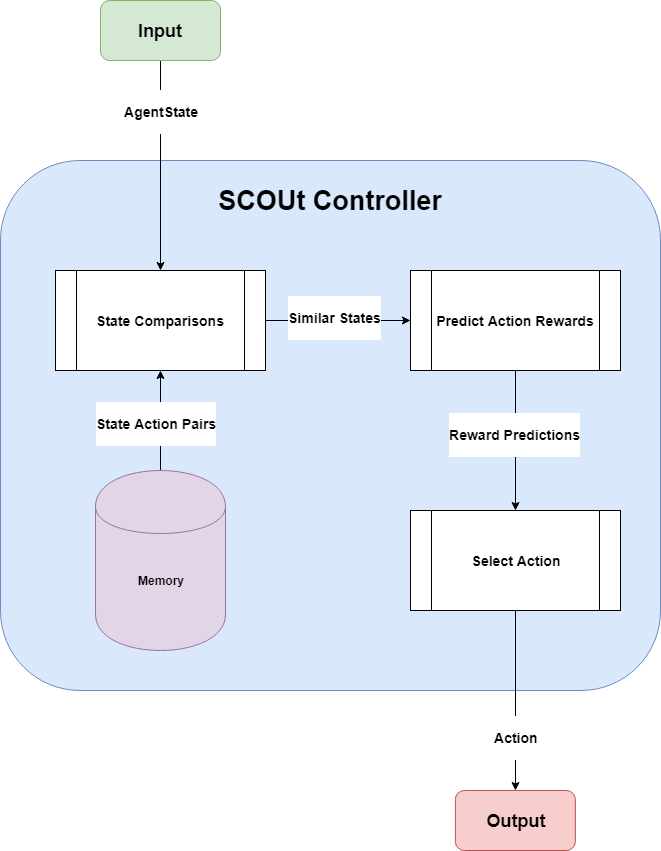
\includegraphics[width=1.0\columnwidth]{Figures/SCOUt_action_decision_model.png}
  \caption{Action decision model for the SCOUt controller.}
  \label{fig:SCOUt_decision_model}
\end{figure}

Calculations used for action decisions rely on several weights to assist in state comparisons and decision making processes.
Because of the large number of weights required for these calculations, a basic genetic algorithm (GA) was used to generate and evolve different sets of weights.
The GA initialized a population of 10 weight sets and evolved them for 50 generations.
Each generation creates five mutated copies and five crossover copies of individuals in the current population.
The individual(s) that are copied for mutation or crossover are chosen using roulette selection. \todo{ref roulette selection?}
Fitness scores are calculated for each of the resulting 20 individuals based on their performance within a series of 50 operations.
Ten survivors are then selected for the next generation.
Survivor selection keeps the two individuals with the highest fitness scores, and uses roulette selection for choosing the remaining seven.
The weight set with the highest fitness in the final generation was selected for use in experimentation, and are listed in table ~\ref{table:evolved_weight_set}.

\todo{ref table}
\begin{center}
  \label{table:evolved_weight_set}
  \caption{Table ~\ref{table:evolved_weight_set}: Evolved Weight Set}
  \caption{Set of values and weights used by the SCOUt controller for action selection. These values/weights were produced using a GA.}
  \begin{tabular}{ l l c }
    \textbf{Attribute}                & \textbf{Use}                    & \textbf{Value/Weight} \\
    \hline
    similarityThreshold               & state comparison qualification  & 0.26  \\
    health                            & state comparison                & 0.41  \\
    energy                            & state comparison                & 0.78  \\
    elementState                      & state comparison                & 0.61  \\
    quadrantStates                    & state comparison                & 0.16  \\
    elementState.indicator            & state comparison                & 0.31  \\
    elementState.hazard               & state comparison                & 0.07  \\
    elementState.percentKnownInRange  & state comparison                & 1.0   \\
    elementState.immediateKnown       & state comparison                & 0.41  \\
    quadrantState.indicator           & state comparison                & 0.38  \\
    quadrantState.hazard              & state comparison                & 0.23  \\
    quadrantState.percentKnown        & state comparison                & 0.2   \\
    quadrantState.averageValue        & state comparison                & 0.19  \\
    quadrantState.immediateValue      & state comparison                & 0.29  \\
    minimumSimilarStates              & confidence calculation          & 10    \\
    repetitionPenalty                 & action selection                & 0.1   \\
    predictedShortTermReward          & movement action selection       & 0.87  \\
    predictedLongTermReward           & movement action selection       & 0.45  \\
    confidence                        & movement action selection       & 0.25  \\
    predictedShortTermReward          & scanning action selection       & 0.61  \\
    predictedLongTermReward           & scanning action selection       & 0.34  \\
    confidence                        & scanning action selection       & 1.0   \\
    \hline
  \end{tabular}
\end{center}


\subsection{Memory}
Memory can be gathered from every operation that the SCOUt controller is used in.
When an operation has finished, and long term rewards have been assigned to each action, the controller creates new state-action pairs, and selects a sub-set of them to be stored in memory.
Saving only a sub-set cuts back on the size of the memory file and the computational time required while searching for similar states.
The current memory selection method in this project saves the last 20 SAPs, and a uniformly sampled sub-set of remaining SAPs from the operation.
The last 20 are always saved because they typically hold the most important events leading up to the success or failure of the operation.
Five percent of the remaining SAPs are uniformly sampled so that the memory will also contain information related to the agent's initial and intermediate search behavior.
Each state-action pair is added to the controller's memory file as a Json object.
The collection of SAPs can then be decoded from the file the next time the controller's memory is loaded.


\subsection{State Normalization}
SCOUt begins each operation by loading in all \texttt{StateActionPair}'s from memory.
The data within each SAP's state is relative to the operation they were recorded in.
To handle the variances found between all of these states, SCOUt normalizes them using a Gaussian approach suggested by McCaffrey \cite{mccaffrey_how_nodate}.
Normalization helps make data values more meaningful when studied by the controller.
For example, if the controller was seeking out a human, it may look for increases in decibel values.
In order for the controller to determine how much of an increase is significant enough to investigate, it needs to first understand what variations are considered normal.
Gaussian distribution provides this functionality through the calculation of average and standard deviation (SD) values in a data set.
If the agent has gathered decibel readings in its north quadrant that are well outside the SD, it should be encouraged to investigate.
All numerical attributes within an \texttt{AgentState} are normalized using this Gaussian method.
This applies to each of the following attributes:

\begin{itemize}
\item \texttt{health}
\item \texttt{energyLevel}
\item \texttt{elementState[$0 - n$].percentKnownInSensorRange}
\item \texttt{elementState[$0 - n$].quadrantState[$N,S,W,E$].percentKnown}
\item \texttt{elementState[$0 - n$].quadrantState[$N,S,W,E$].averageValueDifferential}
\item \texttt{elementState[$0 - n$].quadrantState[$N,S,W,E$].immediateValueDifferential}
\end{itemize}

First, each attribute type is extracted from all SAP states within the loaded memory.
Next the mean and standard deviation values are calculated and stored in an instance of a \texttt{GuassianData} class ~\ref{code:GaussianData}.
Once mean and standard deviation values are known, the controller will go back through every SAP state and normalize their attribute using each corresponding \texttt{GaussianData} set.
The normalization function ~\ref{eq:gaussianNormalize} will produce a "normal" value that reflects how many standard deviations the attribute falls above or below the mean.
A value of 0 represents no difference between the attribute's value and the mean.
Values of 1 and -1 represent a difference of one standard deviation from the mean, and so on.
When SCOUt searches for similar states, it will also normalize the current state using the existing sets of Gaussian data.
By normalizing the current state to memory states, the numerical attributes compared will all be relative to the existing memory pool.

\todo{normalization eq}
\caption{Normalization of an attribute value, $x$, based on the gaussian mean, $m$, and gaussian standard deviation, $sd$, for the given attribute.}
\begin{equation} \label{eq:gaussianNormalize}
  x_{normal} = \frac{(x - m)}{sd}
\end{equation}



\subsection{State Comparisons}
Now that all state attributes are normalized, the controller can use a more intuitive approach for calculating differences between two states.
Several difference comparisons are used to build a collection of state-action pairs that contain states similar to the current state.
These SAPs will later be used to assist in reward prediction.
For an SAP to be considered during reward prediction, it must have an overall difference below the \textit{similarityThreshold} specified in table ~\ref{table:evolved_weight_set}.
Overall state difference is calculated using a series of differences between state attributes, which will all be averaged using a weighted average (equation ~\ref{eq:weighted_average}).
Comparing attributes within \texttt{AgentState} separately allows the controller to assign a level of importance to each one through the use of weights (found in table ~\ref{table:evolved_weight_set}).
Weight values are between 0 and 1.
The higher the attribute's weight it, the more influence it will have in the overall difference.
An attribute with a weight of 0 will be completely ignored in a weighted average equation.
Different weighted average equations are used for overall state difference calculation when the considered SAP's action is movement or scanning type.
This allows the controller to compare only attributes that are relevant to the action that was taken.

\caption{A general equation that takes a list of $n$ attribute values ($V$) and a list of $n$ corresponding weights ($W$) and calculates a weighted average of all attribute values.}
\begin{equation} \label{eq:weighted_average}
  WeightedAverage = \frac{\sum_{i=0}^{n} A_{i} * W_{i}}{\sum_{i=0}^{n} W_{i}}
\end{equation}

Difference comparisons for each attribute in an \texttt{AgentState} are calculated based on their data type (boolean value, normalized numerical value, or sub-class).
Sub-class comparisons, such as comparing two \texttt{ElementState}s, follow the same procedure as \texttt{AgentState}.
Difference comparisons will be made for each of the attributes within the sub-class, and a weighted average equation ~\ref{eq:weighted_average} function is applied to the results.
Boolean differences will return 1 when the compared attributes are both true or both false, and return 1 otherwise.
For example, \textit{BooleanDifference} is used to calculate whether an element type in two states were both flagged as an indicator or not.
Normalized numerical attributes follow the \textit{GaussianDifference} equation ~\ref{eq:gaussian_difference}.
This equation will produce values that hold the same principal as the normalization process, where the closer the difference is to 0, the more similar they are.
If two values are identical, their Gaussian difference will be 0.
Otherwise, the \textit{GaussianDifference} will be relative to how many standard deviations away from each other the two values are.
Proofs for these behaviors are found in appendix item ~\ref{proof:gaussian_difference_identical} and appendix item ~\ref{proof:gaussian_difference_different} respectively.

\caption{Difference calculation for two boolean values, $x$ and $y$.}
\begin{equation}
  BooleanDifference = \begin{cases}
  x = y & 0 \\
  x \neq y & 1
\end{cases}
\end{equation}

\caption{Difference calculation for two normalized vales, $x$ and $y$.}
\begin{equation} \label{eq:gaussian_difference}
  GaussianDifference = |x_{normal} - y_{normal}|
\end{equation}


Comparisons with SAP's whose chosen action was a scanning action factor in the health, energy, and element state differences from each of the \texttt{AgentState}s (equation ~\ref{eq:scanning_overall_difference}).
Each \texttt{ElementState} within the current \texttt{AgentState} will calculate an \textit{elementStateDifference} using its own equation ~\ref{eq:element_state_difference}.
All of these \textit{elementStateDifference}s will be averaged (non-weighted) into a single difference value, \textit{averageElementStateDifference}.
Difference between two \texttt{ElementState}s compares the usage of the element type (hazard and/or indicator detection), and knowledge of the element type (percent known values).
The \textit{hazard} and \textit{indicator} differences can help the controller determine the importance and usage of the element type's data being collected.
The \textit{percentKnown} and \textit{immediateValuesKnown} differences help the controller decide whether usage of an element type's sensor is efficient, or necessary.
For example, if an agent does not have knowledge of the Elevation in adjacent cells, it couldn't confidently determine whether moving into one of those cells would result in a successful move without taking damage.

\caption{Calculation for the overall state difference when the compared state-action pair had chosen a scanning action, where $V$ is a list of attributes values and $W$ is the list of weights for the attributes.}
\begin{equation} \label{eq:scanning_overall_difference}
  V = {health_{diff}, energy_{diff}, averageElementStateDifference_{diff}} \\
  W = {health_{wight}, energy_{wight}, averageElementStateDifference_{wight}} \\
  \\
  OverallDifference_{s} = WeightedAverage(V,W)
\end{equation}

If the action type is movement, overall state difference is calculated using health, energy, element state differences, and quadrant differences (equation ~\ref{eq:movement_overall_difference}).
In addition to calculating an \textit{averageElementStateDifference}, quadrant-to-quadrant differences are calculated between every quadrant in the current state, and every quadrant in the SAP state.
Only one "orientation" of quadrant-to-quadrant comparisons will be used in the overall difference calculation.
Four orientations are considered by rotating the SAP's quadrants in 90 degree intervals (see figure ~\ref{fig:quadrant_orientations}).
The resulting orientation are denoted as North-to-North, North-to-West, North-to-South and North-to-East.
An average of the \textit{quadrantToQuadrantStateDifference} values in each orientation is then calculated, and the orientation with the lowest average difference is used for calculating $OverallDifference_{m}$.

\caption{Calculation for the overall state difference when the compared state-action pair had chosen a scanning action, where $V$ is a list of attributes values and $W$ is the list of weights for the attributes.}
\begin{equation} \label{eq:scanning_overall_difference}
  V = {health_{diff}, energy_{diff}, averageElementStateDifference_{diff}, lowestQuadrantOrientationDifference_{diff}} \\
  W = {health_{wight}, energy_{wight}, averageElementStateDifference_{wight}, lowestQuadrantOrientationDifference_{weight}} \\
  \\
  OverallDifference_{s} = WeightedAverage(V,W)
\end{equation}

\begin{figure}[h]
  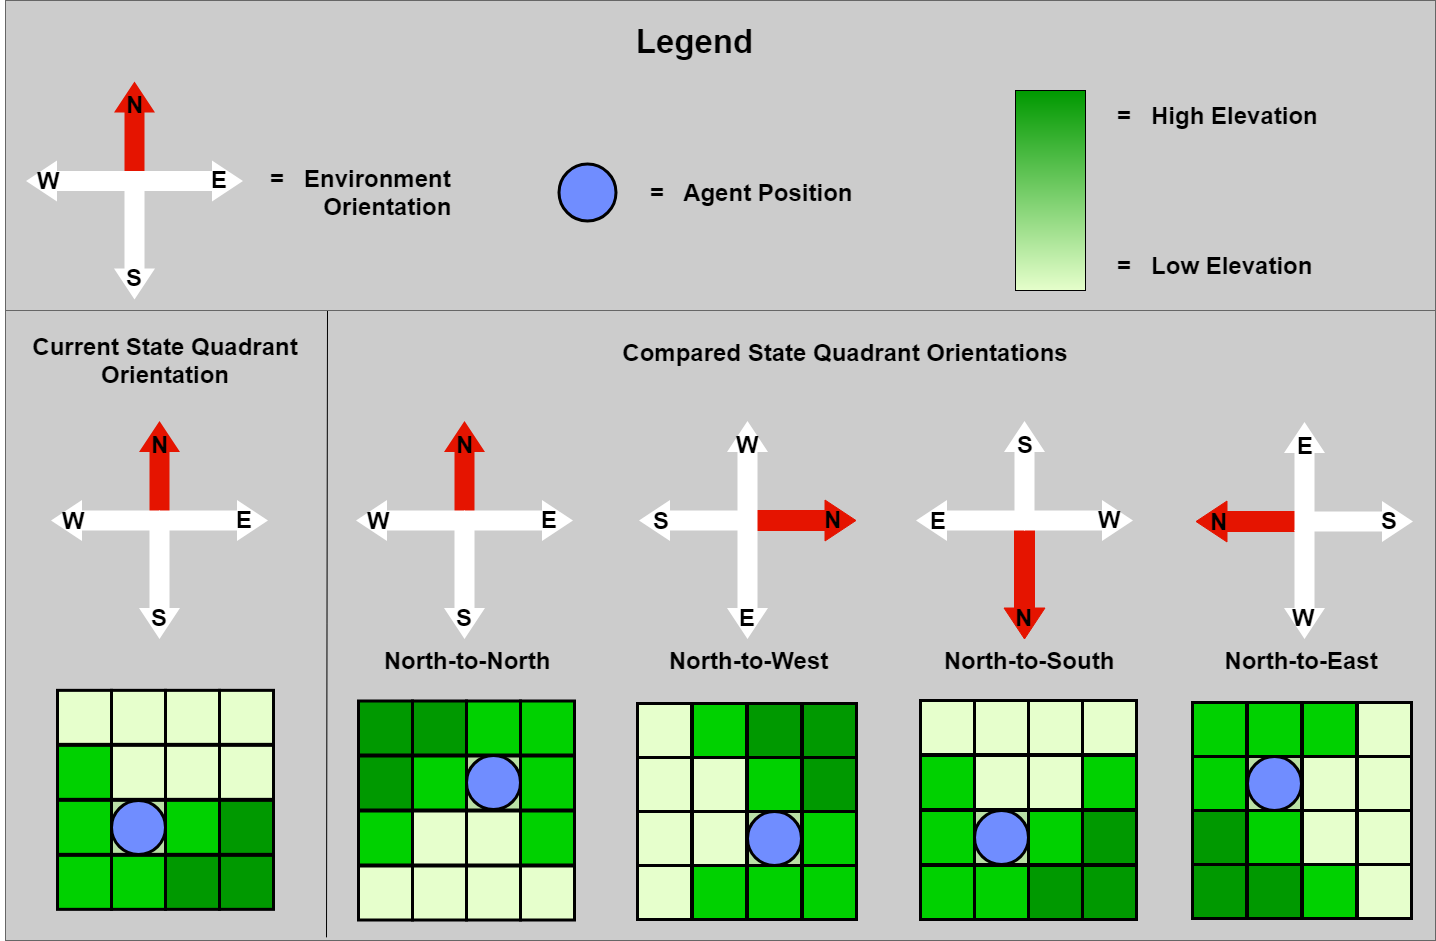
\includegraphics[width=1.0\columnwidth]{Figures/quadrant_orientations.png}
  \caption{Orientation considerations between two compared states.}
  \label{fig:quadrant_orientations}
\end{figure}

Each orientation is important to consider because the controller is only concerned with moving towards interesting features in an Environment, regardless of the direction.
Considering the orientation with the lowest difference makes the comparison relative to the environments instead of the directionality.
Consider an SAP's whose highest matching orientation is found when rotating the quadrants 180 degrees (North-to-South orientation).
If the SAP held record that the agent received a high reward for their movement action, the current agent should be encouraged to move towards a quadrant with similar features (not necessarily in the same direction).
So if the SAP's agent had chosen to move East in its environment, the current agent should choose to move West in their environment since the two states were most similar in the North-to-South orientation.


Quadrant-to-quadrant comparisons produce a non-weighted average of attribute differences in each of the corresponding \textit{QuadrantState}s between the current state's list of \texttt{ElementState}s and the matching \texttt{ElementState} in the SAP state.
These comparisons are denoted as \textit{quadrantElementStateDifference}s, as they only consider one quadrant of each \texttt{ElementState}.
For example, making a North-to-South quadrant comparison would consider data in the current states North quadrant against data in the SAP's South quadrant.
When making these comparisons, it is not guaranteed that the current state and SAP state will share all of the same types of \texttt{ElementState}s.
If the current state contains Decibel data and the SAP state does not, it will receive a \textit{quadrantElementStateDifference} of 1.
Because we are only comparing against \texttt{ElementState}s in the current \texttt{AgentState}, if the SAP contains any \texttt{ElementState}s not present in the current state, they are simply ignored.
These comparisons use equation ~\ref{ea:quadrant_element_state_difference} to examine how much data about the element type is known, and the actual values that are known.
Because \texttt{averageValueDifferential} and \texttt{immediateValueDifferential} are both \texttt{Option[Double]}, they have a unique difference equation (equation ~\ref{eq:option_difference}).

\caption{Calculation for comparing the difference between two \texttt{ElementState}s in a given quadrant, where $V$ is a list of attributes values and $W$ is the list of weights for the attributes.}
\begin{equation} \label{eq:scanning_overall_difference}
\begin{align}
  &V = \{percentKnown_{diff},\quad averageValueDifferential_{diff},\quad immediateValueDifferential_{diff}\} \\
  &W = \{percentKnown_{wight},\quad averageValueDifferential_{wight},\quad immediateValueDifferential_{wight}\} \\
  &\\
  &OverallDifference_{s} = WeightedAverage(V,W)
\end{align}
\end{equation}

\caption{A difference calculation used for two values ($x$ and $y$), where the values are not always known.}
\begin{equation} \label{eq:option_difference}
  difference = \begin{cases}
    x \quad \text{known} \cap y \quad \text{known} & GaussianDifference(x,y) \\
    x \quad \text{known} \cup y \quad \text{known} & 1 \\
    x \quad \textbf{NOT} \quad \text{known} \cap y \quad \textbf{NOT} \quad \text{known} & 0
\end{cases}
\end{equation}


If the calculated overall difference is below the \textit{similarityThreshold}, an instance of the \texttt{StateActionDifference} class (code ~\ref{code:state_action_difference}) is created for use in reward prediction.
Each instance stores the overall difference value, the SAP's action taken, and the short and long term rewards.
State comparison will be repeated for every SAP in the memory pool, and the resulting collection of \texttt{StateActionDifference} instances is passed to the action reward prediction algorithm.

\begin{lstlisting} \label{code:state_action_difference}
class StateActionDifference(
  overallStateDifference: Double
  action: String
  shortTermScore: Double
  longTermScore: Double
)
\end{lstlisting}


\subsection{Action Reward Prediction}
Once the controller has found a set of SAPs with similar states, it will predict a short and long term reward value that each possible action might receive if the agent choses it, along with a confidence score for each one.
For each valid action considered, the algorithm will select a sub-set of the \texttt{StateActionDifference}s where the \texttt{action} is the same as the one being considered.
Predicted short and long term rewards are calculated as an average of all the \texttt{shortTermScore}s and \texttt{longTermScore}s in the sub-set respectively.
Confidence is evaluated using the average of all \texttt{overallStateDifference}s in the sub-set, but is weighted based on the number of \texttt{StateActionDifference}s in the sub-set (equation ~\ref{eq:confidence}).
The equation will invert \textit{overallStateDifference}s when averaging them by subtracting their value from 1.
This allows the prediction algorithm to look at them as "similarity" scores instead of "difference" scores.
Two identical states will then have a similarity score of 1.
Because \textit{similarityThreshold} was used to filter out SAPs with high overall difference values, it will be assured that the sum of all \textit{overallStateDifference}s will not fall below $1 - similarityThreshold$.
The prediction algorithm then computes an overall score for the action using a weighted summation of the predicted short and long term rewards, and the confidence score (equation ~\ref{eq:action_score}).

\caption{Confidence value assigned to reward prediction values based on a set of $n$ \texttt{StateActionDifference}s ($SAD$), and the $minimumSimilarStates$ value from the evolved weight set (table ~\ref{table:evolved_weight_set}).}
\begin{equation} \label{eq:confidence}
  confidence = \begin{cases}
    n = 0 & 0 \\
    n < minimumSimilarStates & \frac{\sum_{n}{i=0} 1 - SAD_{i}.overallStateDifference}{minimumSimilarStates} \\
    n >= minimumSimilarStates & \frac{\sum_{n}{i=0} 1 - SAD_{i}.overallStateDifference}{n} \\
\end{cases}
\end{equation}

\caption{Action scoring function using the action's $predictedShortTermReward$, $predictedLongTermReward$, and $confidence$, in pairing with their corresponding weights found in table ~\ref{table:evolved_weight_set}}
\begin{equation} \label{eq:action_score}
  &V = \{predictedShortTermReward,\quad predictedLongTermReward,\quad confidence\} \\
  &W = \{predictedShortTermReward_{weight},\quad predictedLongTermReward_{weight},\quad confidence_{weight}\} \\
  &\\
  &actionScore = WeightedAverage(V,W)
\end{cases}
\end{equation}


\subsection{Action Selection}
Once every valid action has received an \textit{actionScore}, there are two methods for choosing which one the agent should perform.
If the controller is being trained, roulette selection is used.
Roulette selection is an integral part of training as it will give every action a chance to be selected.
This will fill the controller memory with a variety of events, both good an bad.
when the controller is being used outside of training, the action with the highest score is always selected.
The agent will then attempt to perform the selected action, and its interaction with the environment will then be reflected in a new \texttt{AgentState}.
If the agent is still operational after the resulting event, and the goal has not yet been completed, the action decision process (figure ~\ref{fig:SCOUt_action_decision_model}) will begin again using the new \texttt{AgentState}.
Once the agent is no longer operational, or the goal has been completed, the operation process ends and new SAPs are added to the controller's memory file.






\todo{proof 1}
\begin{lstlisting} \label{proof:gaussian_difference_identical}
Example:
Gaussian mean = 10
Gaussian standard deviation = 1

x = 12
y = 12
x = y

x(normalized) = (x - Gaussain mean) / Gaussian standard deviation
x(normalized) = (12 - 10) / 1
x(normalized) = 2 / 1
x(normalized) = 2

y(normalized) = (y - Gaussain mean) / Gaussian standard deviation
y(normalized) = (12 - 10) / 1
y(normalized) = 2 / 1
y(normalized) = 2

x(normalized) = y(normalized)

Gaussian difference (x,y) = |x - y|
Gaussian difference (x,y) = |2 - 2|
Gaussian difference (x,y) = 0
\end{lstlisting}


\todo{proof 2}
\begin{lstlisting} \label{proof:gaussian_difference_identical}
Example:
Gaussian mean = 10
Gaussian standard deviation = 1

x = 12
y = 7

x(normalized) = (x - Gaussain mean) / Gaussian standard deviation
x(normalized) = (12 - 10) / 1
x(normalized) = 2 / 1
x(normalized) = 2

y(normalized) = (y - Gaussain mean) / Gaussian standard deviation
y(normalized) = (7 - 10) / 1
y(normalized) = -3 / 1
y(normalized) = -3

Gaussian difference (x,y) = |x - y|
Gaussian difference (x,y) = |2 - -3|
Gaussian difference (x,y) = 5
\end{lstlisting}



% \todo{style algo}
% \begin{lstlisting}
% 1. Normalize the current state (how many SDs it falls outside of the average)
% 2. Calculate the Gaussian difference for:
%   a. health
%   b. energyLevel
%   c. elementStateDifferences = for each element state:
%     i. hazardDifference = if (current == SAP) 1 else 0
%     ii. indicatorDifference = if (current == SAP) 1 else 0
%     iii. percentKnownInSensorRangeDifference = abs(SAP - current)
%     iv. immediateValuesKnownDifference = abs(SAP - current) / 4
%   d. quadrantToQuadrantStateDifferences = for each current quadrant:
%     i. quadrantStateDifferences = for each SAP quadrant:
%       a. quadrantElementStateDifferences = for each element type:
%         i. hazardDifference = if (current == SAP) 1 else 0
%         ii. indicatorDifference = if (current == SAP) 1 else 0
%         iii. percentKnownDifference = abs(SAP - current)
%         iv. averageValueDifferentialDifference = if (current known && SAP known) abs(SAP - current) else (if current known == if SAP knonw) 1 else 0)
%         v. immediateValueDifferentialDifference = if (current known && SAP known) abs(SAP - current) else (if current known == if SAP knonw) 1 else 0)
% 3. Sum all differences together using weighted values for each Gaussian difference.
%   a. Movement state difference
%   b. Scan state difference
% \end{lstlisting}



% \subsection{Action Reward Prediction}
% Action reward prediction first calculates three factors for each valid action being considered: predicted short term reward, predicted long term reward and confidence.
% These factors are determined by StateActionDifference that hold the same action as the current action whose reward is being predicted.
% Only a list of similar StateActionDifferences are considered in these calculations.
% This list is made up of StateActionDifferences with an overall difference below a the set minDifferenceThreshold.
% Predicted short and long term rewards are calculated by the average of short and long term scores within the list of similar StateActionDifferences.
%
% If there are no StateActionDifferences in the list, the action being considered will receive a predicted short term reward and long term reward of 0.5 and a confidence of 0.


% An action's short and long term rewards are predicted from the averages of SAPs where: A) the considered action was selected, and B) the state difference from the current state is below a certain threshold.
% In addition to these predicted rewards, we also calculate a confidence value for the predictions.
% \todo{confidence EQ}
% The lower the difference is between the current and SAP states, the higher the confidence will be.
% Additionally, the more SAPs that are considered in the prediction, the more confident the controller can be in the predicted reward.
